%%%%%%%%%%%%%%%%%%%%%%%%%%%%%%%%%%%%%%%%%%%%%%%%%%%%%%%%%%%%%%%%%%%%%%%%
\chapter{Miscellaneous}\label{chap:inprogress}
%%%%%%%%%%%%%%%%%%%%%%%%%%%%%%%%%%%%%%%%%%%%%%%%%%%%%%%%%%%%%%%%%%%%%%%%

\begin{center}
	\begin{minipage}{0.8\textwidth}
		\begin{small}
			This chapter addresses research question \ref{question3}, presents our ongoing works on efficiently dealing with dermoscopic skin lesion hair artifact, custom architecture for Lyme disease image classifier, and an application utilizing our research findings. Contents from this chapter have been used in the following publications:
			\begin{itemize}
				\item \fullcite{Hossain2023} (accepted, Data in Brief journal)
				\item \fullcite{EMSCacnEGC}.  \textsc{url}: \url{https://editions-rnti.fr/?inprocid=1002869}
				\item \fullcite{EMSCacnECCV}. Project Demo. \textsc{url}: \url{https://eccv2022.ecva.net/program/demo-list/}
			\end{itemize}  
		\end{small}
	\end{minipage}
	\vspace{0.5cm}
\end{center}

\minitoc


%%%%%%%%%%%%%%%%%%%%%%%%%%%%%%%%%%%%%%%%%%%%%%%%%%%%%%%%%%%%%%%%%%%%%%%%
\section{Introduction}
%%%%%%%%%%%%%%%%%%%%%%%%%%%%%%%%%%%%%%%%%%%%%%%%%%%%%%%%%%%%%%%%%%%%%%%%
Artificial intelligence-assisted skin lesion analysis is becoming popular nowadays thanks to the advancement in deep learning techniques. However, their performances may be affected by skin hair artifacts. Lesion analysis can benefit from digital hair removal or realistic hair simulation techniques as discussed in Section \ref{sec:research-questions}. An accurate hair mask segmentation dataset is needed to properly benchmark the segmentation algorithms. Moreover, existing researches on skin hair augmentation require a hair mask to generate hair in specified locations. These masks are created using pre-segmented hair masks or random lines or curves \cite{Attia2020}. A well-annotated hair mask dataset will be effective for training generative models to automate the mask generation process. 

We have created the largest publicly available skin lesion hair segmentation mask dataset by carefully annotating 500 dermoscopic images. Compared to the existing datasets, our dataset is free of non-hair artifacts like ruler markers, bubbles, and ink marks. The dataset is also less prone to over and under segmentations because of fine-grained annotations and quality checks from multiple independent annotators. To create the dataset, first, we collected five hundred copyright-free CC0 licensed dermoscopic images covering different hair patterns. Second, we trained a deep learning hair segmentation model on a publicly available weakly annotated dataset. Third, we extracted hair masks for the selected five hundred images using the segmentation model. Finally, we manually corrected all the segmentation errors and verified the annotations by superimposing the annotated masks on top of the dermoscopic images. Multiple annotators were involved in the annotation and verification process to make the annotations as error-free as possible. 

The prepared dataset will be useful for benchmarking and training hair segmentation algorithms as well as creating realistic hair augmentation systems. Our first plan is to train an accurate hair segmentation model utilizing the prepared dataset to extract lots of hair masks from dermoscopic datasets. Then, these masks can be utilized to train a generative model which can automate the process of realistic hair mask generation for the hair augmentation process. Finally, we want to test if hair augmentation can be an effective replacement for hair removal or not.

We are working on a custom convolutional neural network (CNN) architecture targeting the task of classifying erythema migrans (EM) from images. The architecture utilizes findings from our analysis of existing architectures as described in Chapter \ref{chap:Pretraining}. The initial results look promising and we are planning to further improve the architecture with neural architecture search (NAS) and our proposed pre-training strategy.  

The techniques proposed in this thesis have been utilized in a prototype mobile application for assisting with the early diagnosis of Lyme disease. Initial trials with the application are getting positive feedback from the community.

The rest of the chapter is structured as follows: Section \ref{sec:in_progress_hair} describes our ongoing work on efficiently dealing with skin lesion hair artifact; Section \ref{sec:in_progress_archi} presents the custom architecture for EM image classifier, and the work plan to further improve it; Section \ref{sec:in_progress_application} briefly describes the application utilizing findings from the thesis; finally, Section \ref{sec:in_progress_conclu} presents concluding remarks.
%%%%%%%%%%%%%%%%%%%%%%%%%%%%%%%%%%%%%%%%%%%%%%%%%%%%%%%%%%%%%%%%%%%%%%%%
\section{Efficiently Dealing With Dermoscopic Skin Lesion Hair Artifact}\label{sec:in_progress_hair}
%%%%%%%%%%%%%%%%%%%%%%%%%%%%%%%%%%%%%%%%%%%%%%%%%%%%%%%%%%%%%%%%%%%%%%%%
The following subsections describe our prepared dermoscopic skin lesion hair mask dataset and work plan to effectively handle the hair artifact.

%%%%%%%%%%%%%%%%%%%%%%%%%%%%%%%%%%%%%%%%%%%%%%%%%%%%%%%%%%%%%%%%%%%%%%%%
\subsection{A Skin Lesion Hair Mask Dataset With Fine-grained Annotations}
%%%%%%%%%%%%%%%%%%%%%%%%%%%%%%%%%%%%%%%%%%%%%%%%%%%%%%%%%%%%%%%%%%%%%%%%
The following subsections present our motivation behind creating the dataset, value of the data, data description, and methods of dataset preparation.

%%%%%%%%%%%%%%%%%%%%%%%%%%%%%%%%%%%%%%%%%%%%%%%%%%%%%%%%%%%%%%%%%%%%%%%%
\subsubsection{Motivation}
%%%%%%%%%%%%%%%%%%%%%%%%%%%%%%%%%%%%%%%%%%%%%%%%%%%%%%%%%%%%%%%%%%%%%%%%
According to our study, the largest publicly available skin lesion hair mask dataset \cite{Li2021a} contains annotations for 306 images but with 18 duplicates and suffers from under-segmentation, and non-hair artifacts. Gallucci \cite{Gallucci2020} created a dataset of 75 images only, which lacks complex patterns and is not a well-representative of the broader skin hair distribution. Akyel et al. \cite{Akyel2022} prepared a non-public dataset of 2500 images. However, it contains rulers, ink spots, and other noises alongside skin hair. Our motivation for creating the dataset was to resolve the issues in available datasets.

%%%%%%%%%%%%%%%%%%%%%%%%%%%%%%%%%%%%%%%%%%%%%%%%%%%%%%%%%%%%%%%%%%%%%%%%
\subsubsection{Value of the Data}
%%%%%%%%%%%%%%%%%%%%%%%%%%%%%%%%%%%%%%%%%%%%%%%%%%%%%%%%%%%%%%%%%%%%%%%%
\begin{itemize}
	
	\item This is the largest publicly available fine-grained skin lesion hair segmentation mask dataset. High-quality hand-annotated segmentation masks are costly and time-consuming to produce.
	
	\item This is the only dataset free of non-hair artifacts.
	
	\item This dataset will be useful for proper benchmarking of hair segmentation algorithms, as it is free of non-hair artifacts and segmentation errors.
	
	\item Our dataset can be used to train a generative model for automating the task of realistic skin hair mask generation.
	
	\item The dataset will contribute to skin lesion research by allowing researchers to train robust skin lesion hair segmentation algorithms.
	
\end{itemize}


%%%%%%%%%%%%%%%%%%%%%%%%%%%%%%%%%%%%%%%%%%%%%%%%%%%%%%%%%%%%%%%%%%%%%%%%
\subsubsection{Data Description}
%%%%%%%%%%%%%%%%%%%%%%%%%%%%%%%%%%%%%%%%%%%%%%%%%%%%%%%%%%%%%%%%%%%%%%%%
Our dataset is publicly available in an online repository\footnote{\url{https://data.mendeley.com/datasets/j5ywpd2p27} (visited on 02/20/2023).} \cite{Hossain2023}. It contains skin hair annotation masks for 500 dermoscopic images collected from ISIC 2018 dataset \cite{Codella2019}. The dataset is organized into three folders namely dermoscopic\_image, hair\_mask, and overlay. Table \ref{tab:mask_samples} shows some example images from each of the folders. 
\begin{table}[tbh!]
	\centering
	\caption{Samples from the prepared skin lesion hair mask dataset.}
	\label{tab:mask_samples}
	\resizebox{\textwidth}{!}{%
		\begin{tabular}{cccc} 
			\toprule
			& \multicolumn{3}{c}{\textbf{Folder}}        \\ 
			\cmidrule(lr){2-4} 
			\textbf{File}                                   & dermoscopic\_image & hair\_mask & overlay  \\ 
			\midrule
			\begin{sideways}\;\;\;\;\;ISIC\_0000115.png\end{sideways} & 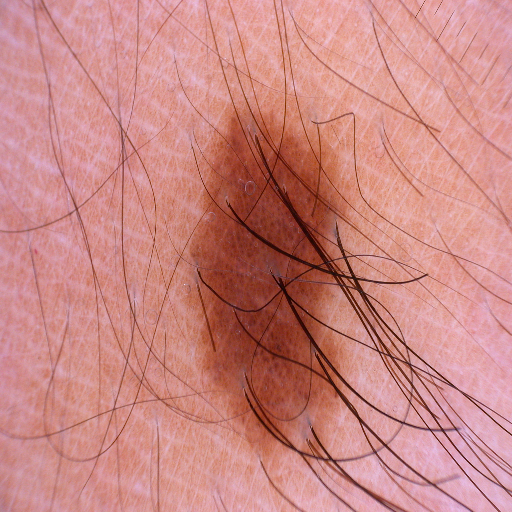
\includegraphics[width=.33\textwidth ,keepaspectratio]{images/ongoing/derm/ISIC_0000115.png}                   &     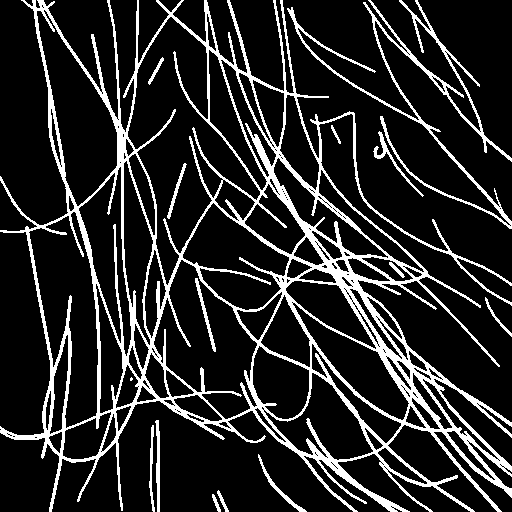
\includegraphics[width=.33\textwidth ,keepaspectratio]{images/ongoing/mask/ISIC_0000115.png}        &     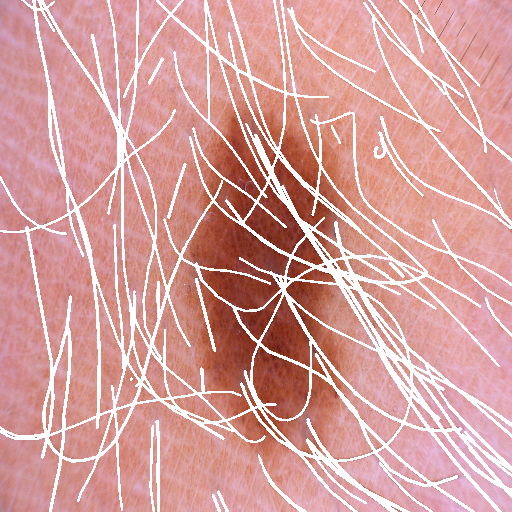
\includegraphics[width=.33\textwidth ,keepaspectratio]{images/ongoing/overlay/ISIC_0000115.png}      \\\cmidrule(lr){1-4} 
			\begin{sideways}\;\;\;\;\;ISIC\_0000200.png\end{sideways} & 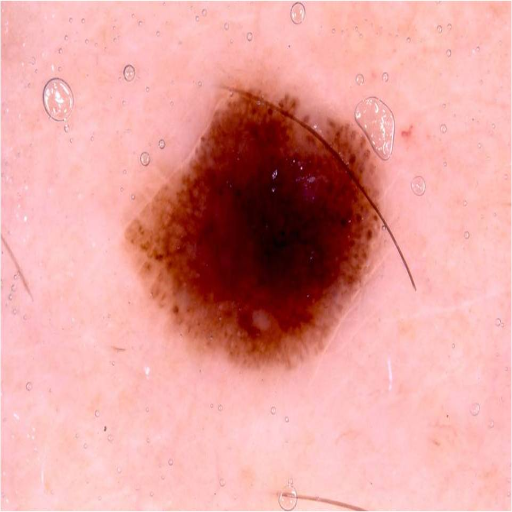
\includegraphics[width=.33\textwidth ,keepaspectratio]{images/ongoing/derm/ISIC_0000200.png}                   &     
\includegraphics[width=.33\textwidth ,keepaspectratio]{images/ongoing/mask/ISIC_0000200.png}        &     
\includegraphics[width=.33\textwidth ,keepaspectratio]{images/ongoing/mask/ISIC_0000200.png}      \\\cmidrule(lr){1-4} 
			\begin{sideways}\;\;\;\;\;ISIC\_0009992.png\end{sideways} & 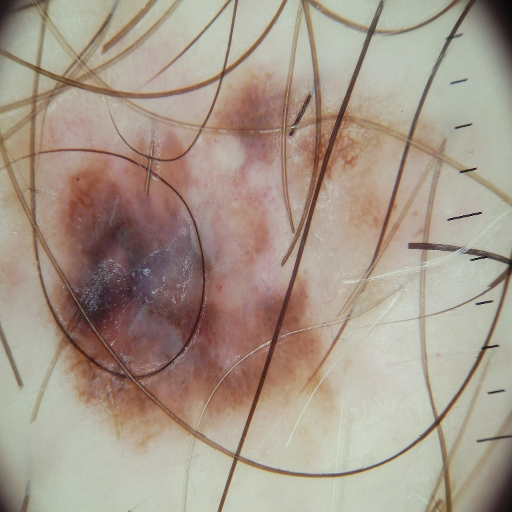
\includegraphics[width=.33\textwidth ,keepaspectratio]{images/ongoing/derm/ISIC_0009992.png}                   &     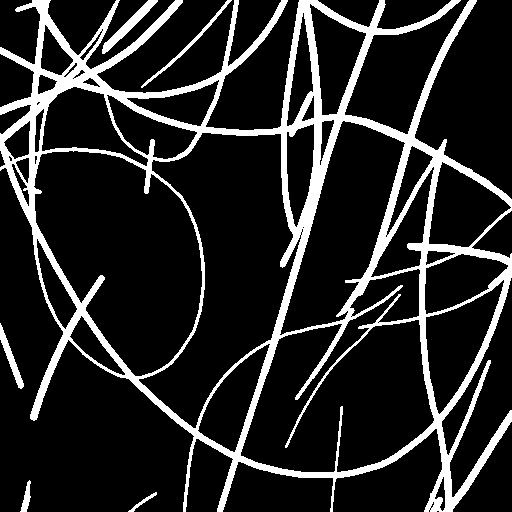
\includegraphics[width=.33\textwidth ,keepaspectratio]{images/ongoing/mask/ISIC_0009992.png}        &     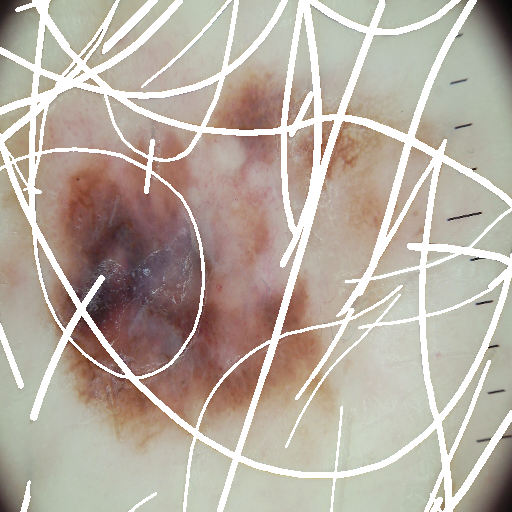
\includegraphics[width=.33\textwidth ,keepaspectratio]{images/ongoing/overlay/ISIC_0009992.png}      \\
			\cmidrule(lr){1-4} 
			\multicolumn{4}{c}{Total: 1500 images (500
				images per folder)}                               \\
			\bottomrule
		\end{tabular}
	}
\end{table}
The dermoscopic\_image folder contains 500 dermoscopic images handpicked from the primary image source covering different hair patterns. We retained the original names of the image files from the primary image source. The hair\_mask folder contains a binary segmentation mask for each of the images of the dermoscopic\_image folder. In a segmentation mask image, white pixels represent skin hair and black pixels represent background. The overlay folder contains hair mask images superimposed on the original dermoscopic images. We provided the superimposed images for easy public verification so that, other people can report any annotation mistakes and contribute to improving the dataset. Images in the hair\_mask and overlay folders share the same names as the primary images in the dermoscopic\_image folder.


%%%%%%%%%%%%%%%%%%%%%%%%%%%%%%%%%%%%%%%%%%%%%%%%%%%%%%%%%%%%%%%%%%%%%%%%
\subsubsection{Dataset Design, Materials and Methods}
%%%%%%%%%%%%%%%%%%%%%%%%%%%%%%%%%%%%%%%%%%%%%%%%%%%%%%%%%%%%%%%%%%%%%%%%
Annotating skin lesion hair from scratch is a tedious task. To ease the process, we trained a U-Net \cite{10.1007/978-3-319-24574-4_28} deep segmentation model using a weakly annotated dataset provided by Li et al. \cite{Li2021a}. U-Net is a popular CNN architecture for image segmentation tasks. It is made up of a contracting path that captures the image's context and an expansive path that creates the segmented output. In order to maintain spatial information, the network uses skip connections, which enables accurate segmentation even when the target objects are small. The U-Net architecture is illustrated in Figure \ref{fig:unet} The codes used for the process are publicly available in the unet folder in a github repository\footnote{\url{https://github.com/imranrana/Skin-Lesion-Hair-Mask-Dataset} (visited on 02/20/2023).\label{note:github_mask}}. Inside the unet folder the U-Net model is defined in model.py file, unet training is performed using the unet\_training.ipynb python notebook file and the task of predicting initial masks for the dermoscopic images are done using the predict\_mask.ipynb file.
\begin{figure}[htb!]
	\centering
	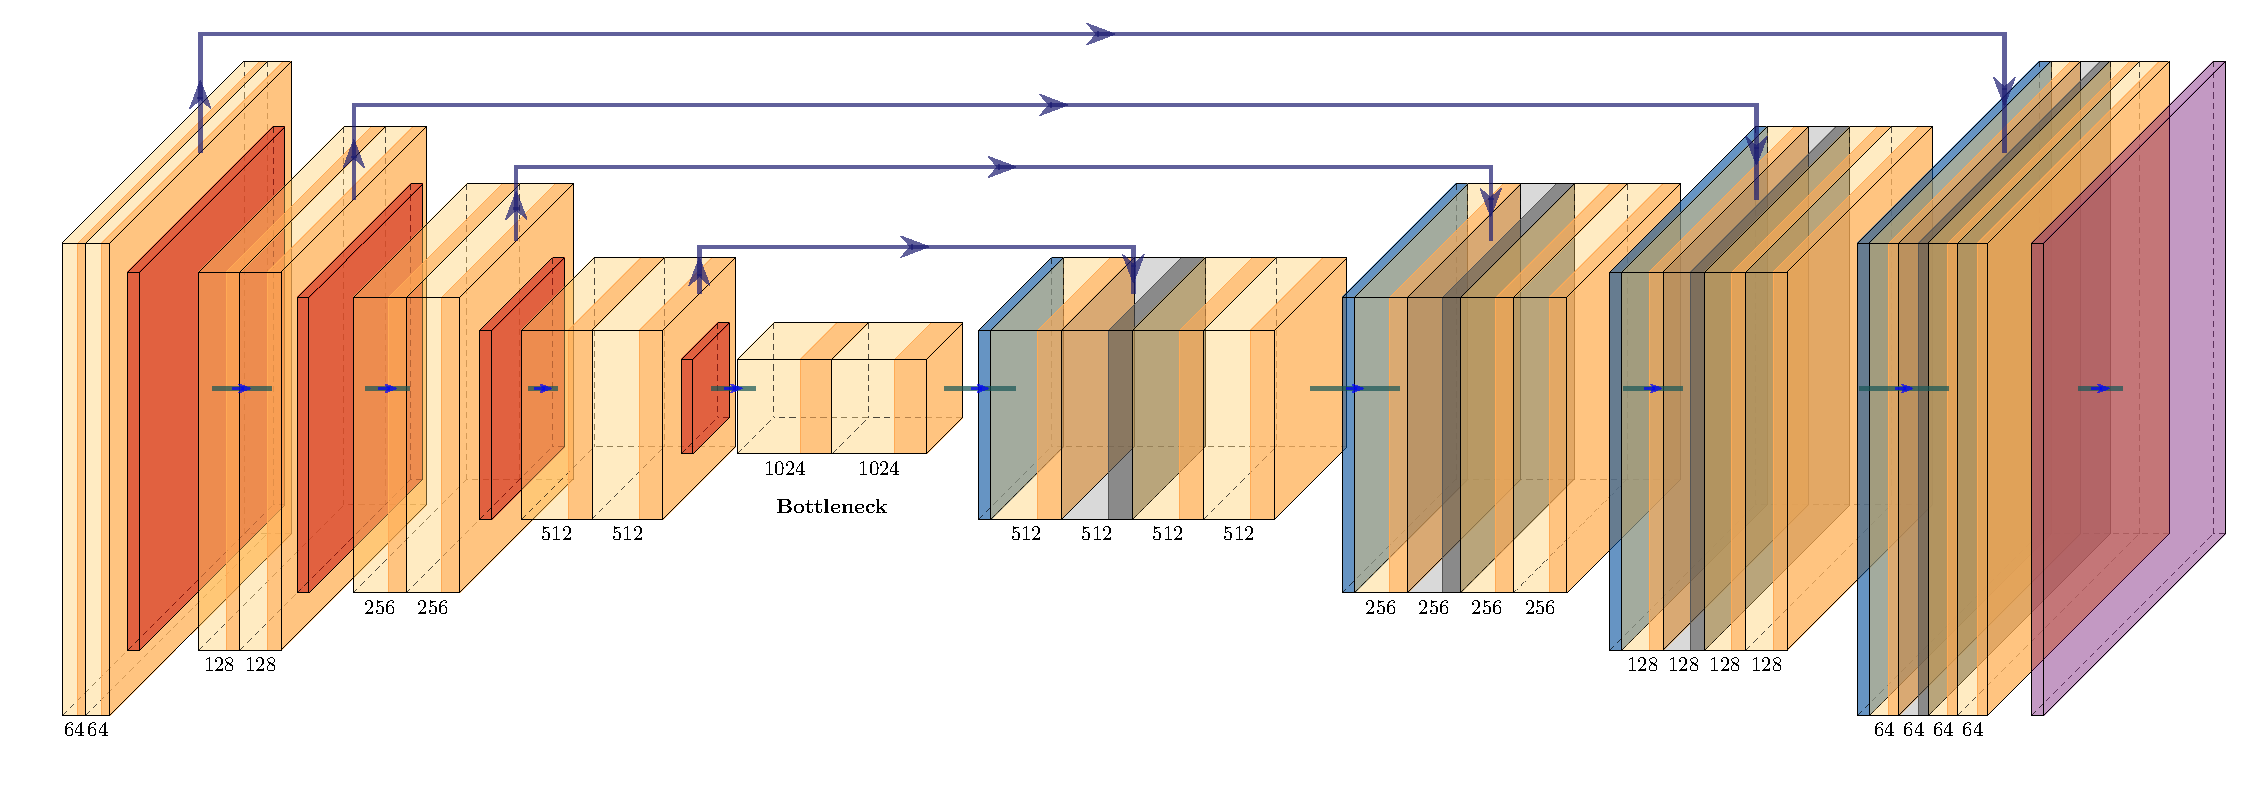
\includegraphics[width=\textwidth,keepaspectratio]{images/ongoing/u-net.pdf}
	\caption[U-Net architecture]{U-Net architecture. The final output layer uses sigmoid activation.}
	\label{fig:unet}
\end{figure}

Using the trained U-Net we extracted the initial hair mask for 500 handpicked copyright-free dermoscopic skin lesion images from ISIC 2018 dataset \cite{Codella2019} to cover different hair patterns. The resulting masks suffer from various segmentation errors like under-segmentation, over-segmentation, and non-hair artifacts. We involved three independent annotators for the correction of the segmentation errors. 

The first annotator manually corrected all the found segmentation errors with Adobe Photoshop software \cite{Photoshop}. A video demonstration of the segmentation mask editing process using Adobe Photoshop software is available in the mask\_editing\_process.mp4 file of our GitHub repository. The steps involved are as follows:
\begin{itemize}
	
	\item Open the dermoscopic image in photoshop.
	\item Open the initial segmentation mask image in photoshop and copy it on top of the dermoscopic image.
	\item Change the blending mode of the mask image to “screen”.
	\item Select the brush type as hard brush (hardness of the brush set to 100 percent).
	\item Remove unwanted segmentation marks from the mask image by painting with a black brush.
	\item Adjust the brush size according to the width of the skin hair and add missing segmentation marks to the mask image by painting with a white brush. 
	\item Change back the blending mode of the mask image to “normal” mode.
	\item Make additional adjustments to the segmentation mask if required.
	\item Save the finalized segmentation mask image in the desired format.
	
\end{itemize}

To verify the quality of the annotation first we binarized each corrected masks to make sure every pixel is either black or white. Then, we made the black pixels of the mask image fully transparent and superimposed it on the original dermoscopic image. Finally, we created a collage of three types of images: dermoscopic image, corrected mask, and the superimposed image for easy verification. Each collage looks like a row from Table \ref{tab:mask_samples}. The code used for these operations is available in the check\_annotation.ipynb file in the github repository\footref{note:github_mask}. Using the image collage a second annotator marked errors missed by the first annotator. A third annotator corrected the mistakes identified by the second annotator, which was finally reverified by the first annotator. We tried to make the annotations as error-free as possible. The overall dataset creation workflow is shown in Figure \ref{fig:mask_data_creation}. 
\begin{figure}[htb!]
	\centering
	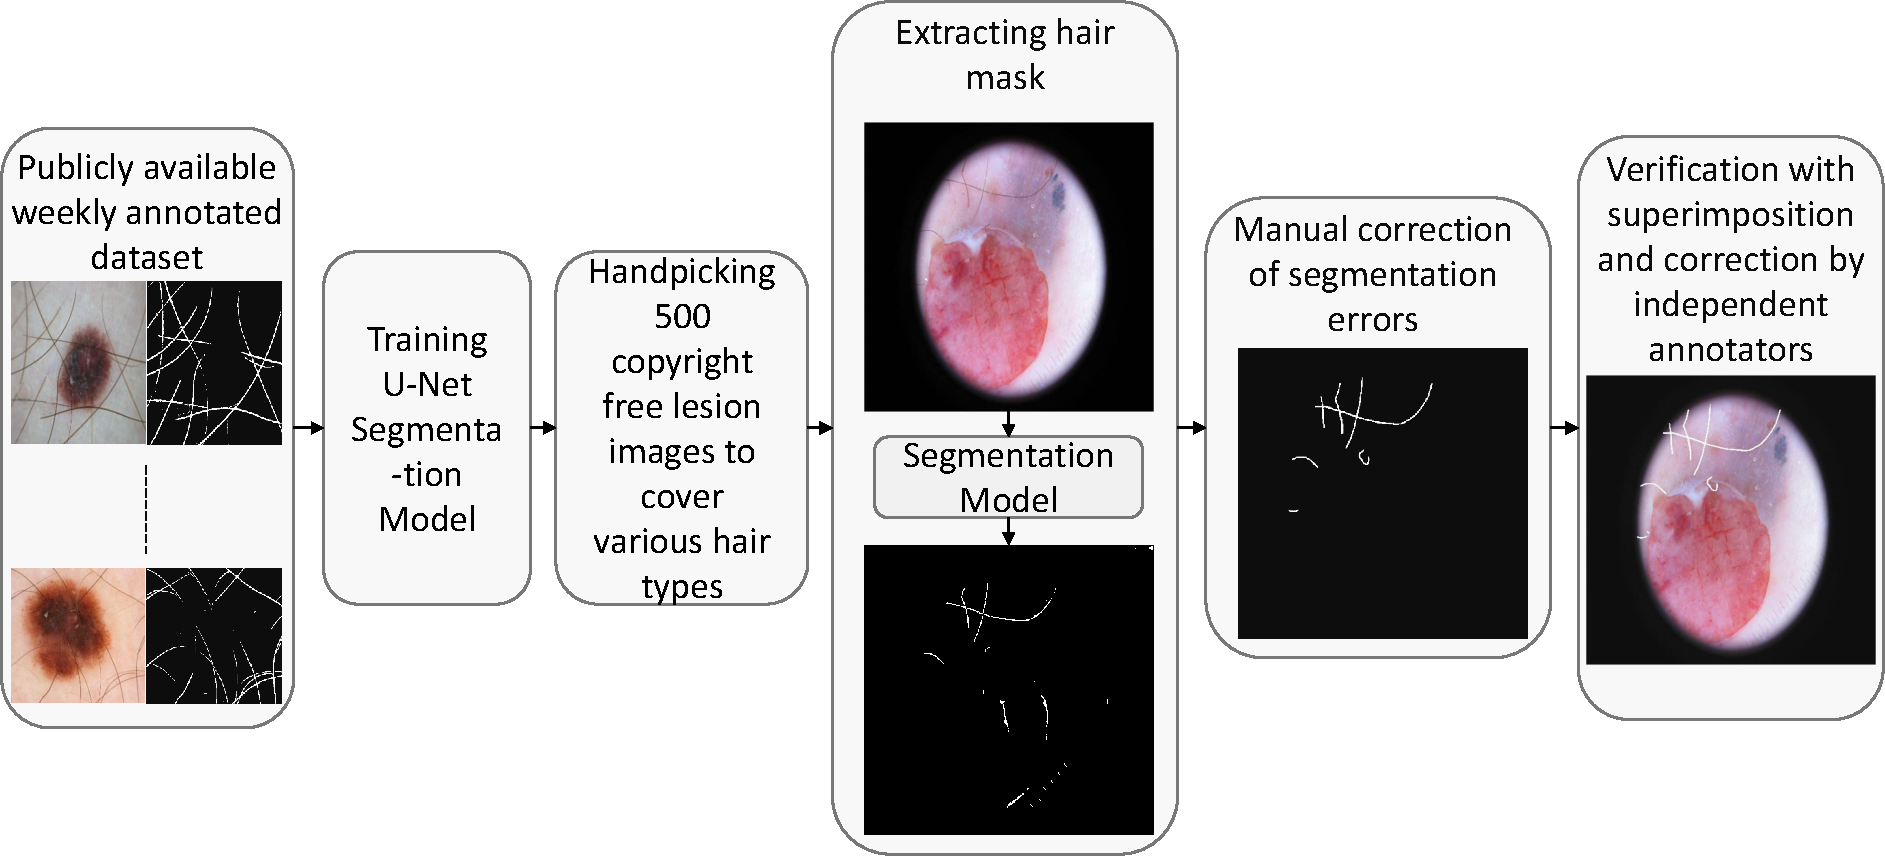
\includegraphics[width=\textwidth,keepaspectratio]{images/ongoing/SkinHair-cropped.pdf}
	\caption{Skin hair mask dataset creation workflow.}
	\label{fig:mask_data_creation}
\end{figure}

%%%%%%%%%%%%%%%%%%%%%%%%%%%%%%%%%%%%%%%%%%%%%%%%%%%%%%%%%%%%%%%%%%%%%%%%
\subsection{Work Plan}\label{sec:hair_plan}
%%%%%%%%%%%%%%%%%%%%%%%%%%%%%%%%%%%%%%%%%%%%%%%%%%%%%%%%%%%%%%%%%%%%%%%%
To address the research question \ref{question3} we want to investigate how augmenting training data with skin hair impacts model performance compared to hair removal. First, we will try to train a generative model to automate the skin hair mask generation process for the augmentation algorithms. If we do not get satisfactory results from the generative model with our created 500 images then, we will train another segmentation model with our dataset and use that model to extract more samples of hair masks from dermoscopic datasets. These images will be useful for the training of the generative model. 

The skin hair augmentation pipeline will work as follows:
\begin{enumerate}[i.]
	\item Remove skin hair from input lesion image with a hair removal algorithm \cite{Li2021a}.
	\item Generate a hair mask with the trained generative model.
	\item Augment hair on the dermoscopic image using the generated mask and a realistic hair simulator \cite{Attia2020}.
\end{enumerate}
We will train a model for dermoscopic image classification using the augmentation pipeline and compare the performance with a model that does not use hair augmentation but uses a hair removal pre-processing step. This study will help to decide if training time hair augmentation can effectively replace test time hair removal pre-processing or not.


%%%%%%%%%%%%%%%%%%%%%%%%%%%%%%%%%%%%%%%%%%%%%%%%%%%%%%%%%%%%%%%%%%%%%%%%
\section{Custom Architecture for Lyme Disease Image Classifier}\label{sec:in_progress_archi}
%%%%%%%%%%%%%%%%%%%%%%%%%%%%%%%%%%%%%%%%%%%%%%%%%%%%%%%%%%%%%%%%%%%%%%%%
From the experimental results discussed in Section \label{sec:pretrain-results}, we saw that ResNet50-141 model performed the best in terms of accuracy for the Lyme disease image classification task and also EfficientNet variations showed good results in heatmap visualization. Taking these factors into consideration we tested a custom architecture as shown in Figure \ref{fig:custom_arch_comb}. We opted for a residual block incorporating efficient channel attention \cite{ECARef} and swish activation as shown in Figure \ref{fig:custom_block}. The architecture design is like a ResNet18 model as shown in Figure \ref{fig:custom_arch}. The source code for the custom architecture is available in a github repository\footnote{\url{https://github.com/imranrana/Lyme-Disease} (visited on 03/15/2023).}. We tested the architecture on the second version of the dataset that includes some label corrections and additional images. The architecture was trained from scratch without any pre-training. The result looks promising compared to the best performing ResNet50-141 model as shown in Table \ref{tab:custom-results}.  The confusion matrix, ROC curve, and cross-validation fold-wise details are available in Appendix Section \ref{sec:app-supply-custom}. The custom architecture has 11.19 million parameters compared to 23.59 million of ResNet50-141. Depthwise separable convolution can be effective in further reducing the parameters but it decreases accuracy. In dilated convolution \cite{dilatedConvRef}, a larger effective kernel size is achieved by introducing gaps, or dilations, between the kernel values as shown in Figure \ref{fig:dilated}. Without increasing the number of parameters or the computational cost, it enables the network to have a bigger receptive field. Combining dilated and depthwise convolutions \cite{Sun2020Dilate} in a residual block (as shown in Figure \ref{fig:dilated_custom_block}) and optimally placing them with the block of Figure \ref{fig:custom_block} utilizing NAS \cite{Ren2021} can produce an effective architecture. Particularly, we plan to use NAS utilizing my previously proposed particle swarm optimization with selective search\footfullcite{ImranHossain2019} for finding the optimized arrangement of these building blocks. Particle swarm optimization with selective search retains the intermediate best result during the particle update process and performs better than vanilla particle swarm optimization. Also, using our proposed pre-training strategy with the architecture may further increase performance.
\begin{figure}[htb!]
	\centering
	\begin{subfigure}[b]{\textwidth}
		\centering
		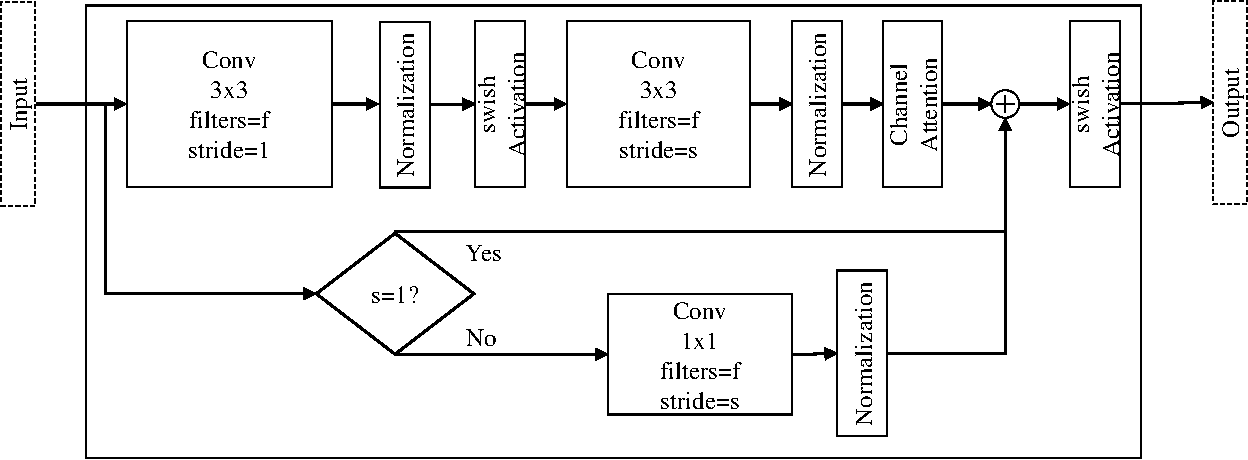
\includegraphics[width=\textwidth,keepaspectratio]{images/ongoing/building_block-cropped.pdf}
		\caption{Building block.}
		\label{fig:custom_block}
	\end{subfigure}
	\hfill
	\begin{subfigure}[b]{\textwidth}
		\centering
		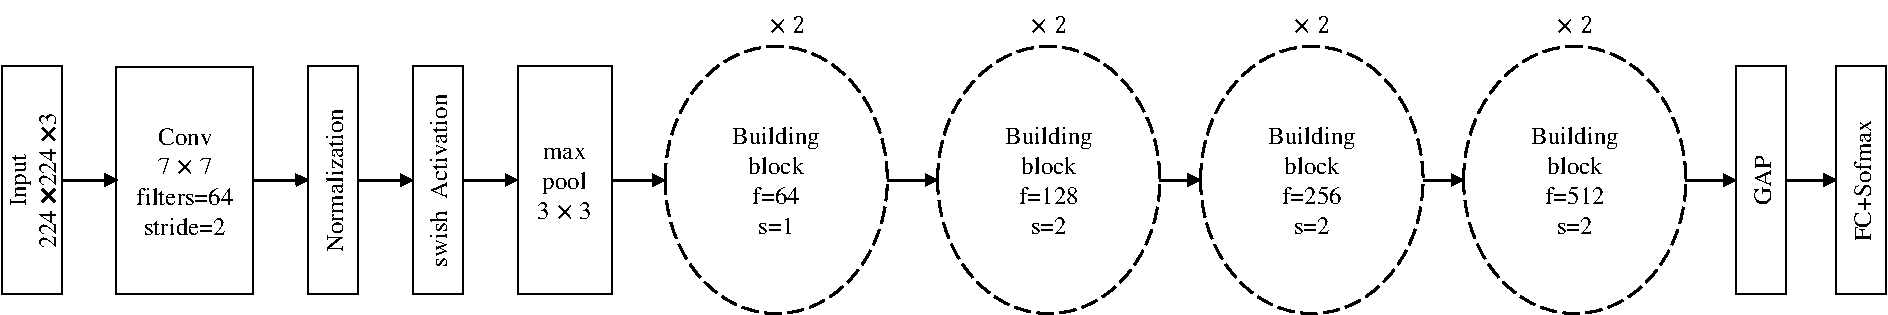
\includegraphics[width=\textwidth,keepaspectratio]{images/ongoing/custom_archi-cropped.pdf}
		\caption{Architecture.}
		\label{fig:custom_arch}
	\end{subfigure}
	
	\caption{Custom architecture design for Lyme image classifier.}
	\label{fig:custom_arch_comb}
\end{figure}
%
\begin{table}[htb!]
	\centering
	\caption[Experimental results with custom architecture]{Experimental results with custom architecture. Within each cell, the value after (±) symbol represents the standard deviation across five folds. Second version of the prepared Lyme dataset was used for the experiments.}
	\label{tab:custom-results}
	\resizebox{\textwidth}{!}{%
		\begin{tabular}{llllllllllll}
			\toprule
			& \multicolumn{11}{c}{\textbf{Metric}}    \\ \cmidrule(l){2-12} 
			\multicolumn{1}{c}{\textbf{Model}} & \rotatebox{45}{Accuracy} & \rotatebox{45}{Sensitivity} & \rotatebox{45}{Specificity} & \rotatebox{45}{Precision} & \rotatebox{45}{NPV} & \rotatebox{45}{MCC} & \rotatebox{45}{Kappa} & \rotatebox{45}{LR$+$} & \rotatebox{45}{LR$-$} & \rotatebox{45}{F1-Score} & \rotatebox{45}{AUC}  \\ \midrule
			ResNet50-141 & \begin{tabular}[c]{@{}l@{}}84.85\\ $\pm$1.23\end{tabular}& \begin{tabular}[c]{@{}l@{}}87.49\\ $\pm$1.83\end{tabular}& \begin{tabular}[c]{@{}l@{}}81.93\\ $\pm$1.42\end{tabular}& \begin{tabular}[c]{@{}l@{}}84.29\\ $\pm$1.09\end{tabular}& \begin{tabular}[c]{@{}l@{}}85.57\\ $\pm$1.89\end{tabular}& \begin{tabular}[c]{@{}l@{}}0.6963\\ $\pm$0.0249\end{tabular}& \begin{tabular}[c]{@{}l@{}}0.6956\\ $\pm$0.0246\end{tabular}& \begin{tabular}[c]{@{}l@{}}4.8707\\ $\pm$0.3856\end{tabular}& \begin{tabular}[c]{@{}l@{}}0.1528\\ $\pm$0.0227\end{tabular}& \begin{tabular}[c]{@{}l@{}}0.8585\\ $\pm$0.0118\end{tabular}& \begin{tabular}[c]{@{}l@{}}0.9231\\ $\pm$0.0069\end{tabular}\\
			\cmidrule(lr){1-12}
			
			Custom & \begin{tabular}[c]{@{}l@{}}84.68\\ $\pm$2.62\end{tabular}& \begin{tabular}[c]{@{}l@{}}87.05\\ $\pm$3.4\end{tabular}& \begin{tabular}[c]{@{}l@{}}82.05\\ $\pm$4.0\end{tabular}& \begin{tabular}[c]{@{}l@{}}84.38\\ $\pm$3.03\end{tabular}& \begin{tabular}[c]{@{}l@{}}85.24\\ $\pm$3.44\end{tabular}& \begin{tabular}[c]{@{}l@{}}0.6936\\ $\pm$0.0526\end{tabular}& \begin{tabular}[c]{@{}l@{}}0.6922\\ $\pm$0.0525\end{tabular}& \begin{tabular}[c]{@{}l@{}}5.1201\\ $\pm$1.2442\end{tabular}& \begin{tabular}[c]{@{}l@{}}0.1582\\ $\pm$0.0434\end{tabular}& \begin{tabular}[c]{@{}l@{}}0.8565\\ $\pm$0.0248\end{tabular}& \begin{tabular}[c]{@{}l@{}}0.9151\\ $\pm$0.0214\end{tabular}\\ 	
			
			\bottomrule
		\end{tabular}%
	}
\end{table}


\begin{figure}[htb!]
	\centering
	\begin{subfigure}[b]{0.5\textwidth}
		\centering
		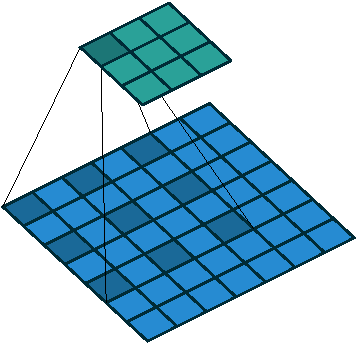
\includegraphics[width=\textwidth,keepaspectratio]{images/ongoing/dilation_00-cropped.pdf}
		\caption{Illustration of dilated convolution \cite{DilatedConv2D}.}
		\label{fig:dilated}
	\end{subfigure}
	\hfill
	\begin{subfigure}[b]{\textwidth}
		\centering
		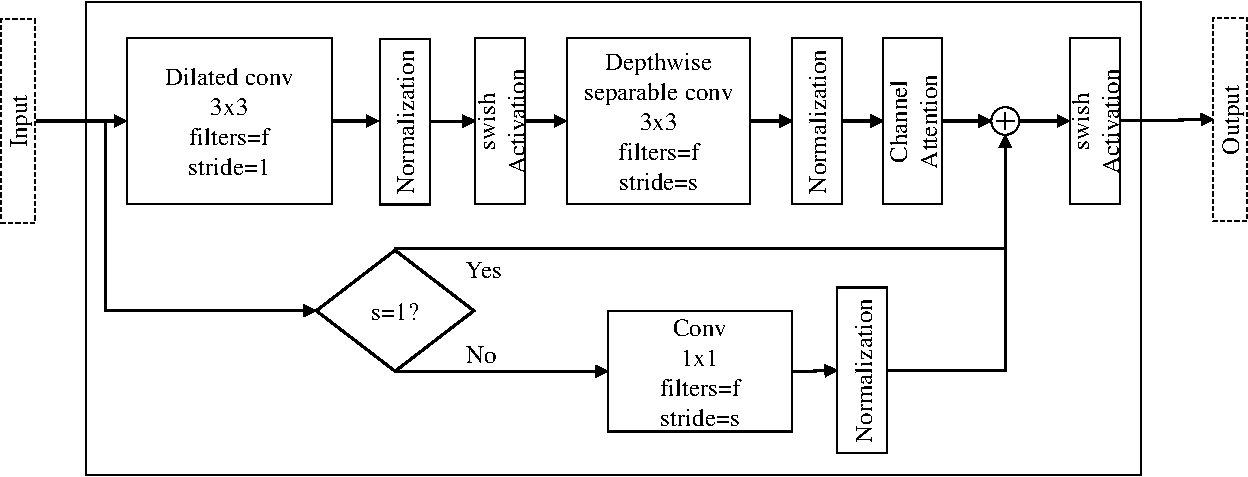
\includegraphics[width=\textwidth,keepaspectratio]{images/ongoing/Dilated_block-cropped.pdf}
		\caption{Custom building block.}
		\label{fig:dilated_custom_block}
	\end{subfigure}
	
	\caption{Custom building block utilizing dilated and depthwise separable convolutions.}
	\label{fig:cust_block_dilated}
\end{figure}

%%%%%%%%%%%%%%%%%%%%%%%%%%%%%%%%%%%%%%%%%%%%%%%%%%%%%%%%%%%%%%%%%%%%%%%%
\section{Application From the Thesis}\label{sec:in_progress_application}
%%%%%%%%%%%%%%%%%%%%%%%%%%%%%%%%%%%%%%%%%%%%%%%%%%%%%%%%%%%%%%%%%%%%%%%%
The techniques proposed in this thesis have been utilized in a mobile application called EMScan. The application was developed as part of the DAPPEM (Développement d’une APPlication d’identification des Erythèmes Migrants à partir de photographies) project funded by European Regional Development Fund. The EMScan mobile application was created with the goal of assisting doctors and general people with early diagnosis and suggestion, and also to advance artificial intelligence assisted Lyme disease diagnosis research. The goals of the application are shown in Figure \ref{EMScan}. Initial trials with the prototype showed promising results for real-life applications. A video demonstration of the application is available on DAPPEM project website\footnote{\url{https://dappem.limos.fr} (visited on 02/20/2023).}. The overall workflow of the EMScan mobile application is described in Appendix Section  \ref{sec:emscan-desc}.
\begin{figure}[htb!]
	\begin{center}
		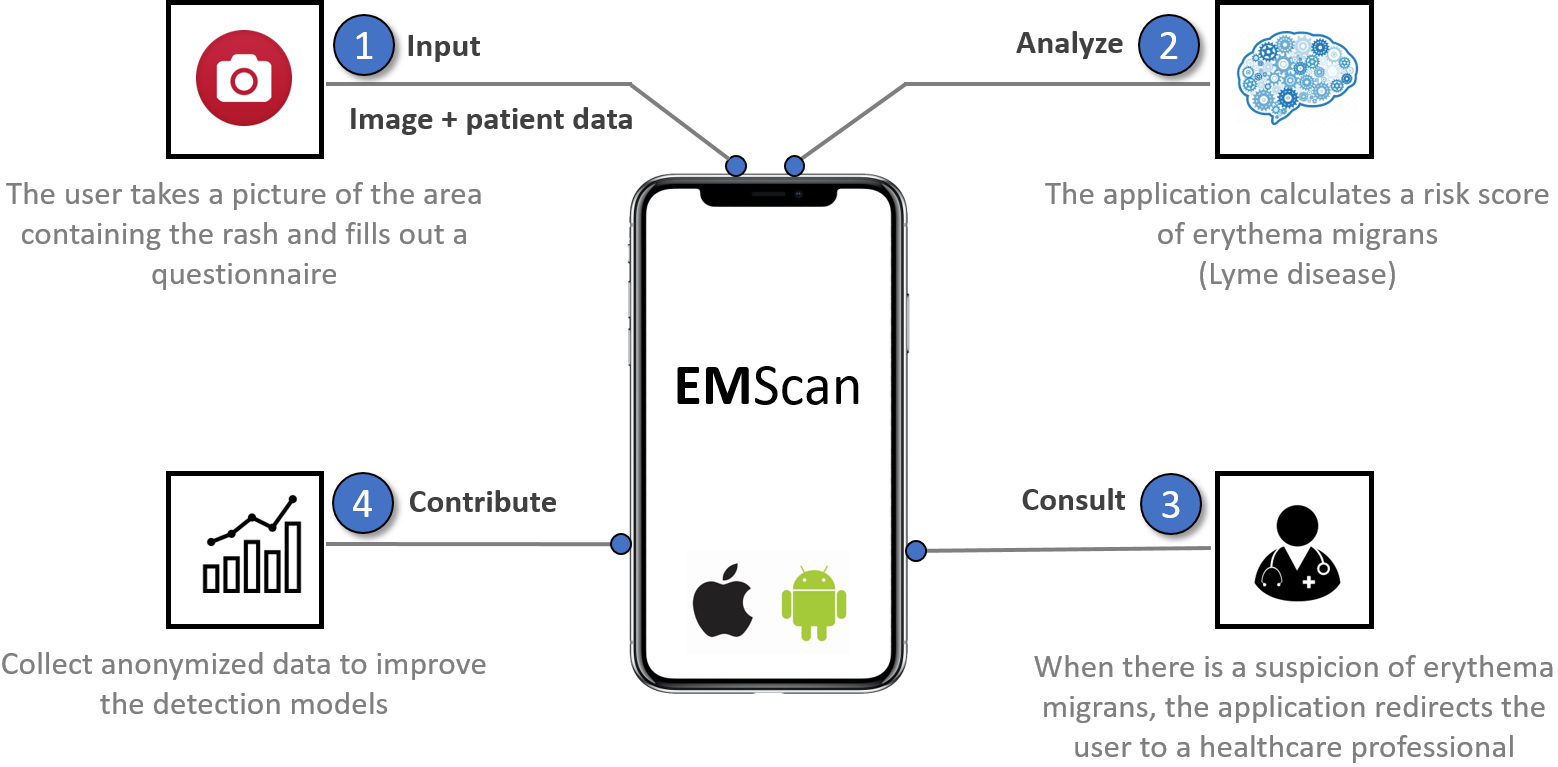
\includegraphics[width=\textwidth,keepaspectratio]{images/ongoing/EMScan.png}
		\caption{EMScan application goals.} \label{EMScan}
	\end{center}
\end{figure}

%%%%%%%%%%%%%%%%%%%%%%%%%%%%%%%%%%%%%%%%%%%%%%%%%%%%%%%%%%%%%%%%%%%%%%%%
\section{Conclusion}\label{sec:in_progress_conclu}
%%%%%%%%%%%%%%%%%%%%%%%%%%%%%%%%%%%%%%%%%%%%%%%%%%%%%%%%%%%%%%%%%%%%%%%%
In this chapter, we have discussed our ongoing research works. We have created the largest publicly available dermoscopic skin lesion hair mask annotation dataset which can be utilized for training accurate segmentation algorithms and also to enhance the hair augmentation process. Further study is required to see if training time hair augmentation can be an effective replacement for test time hair removal or not. We are also working on a custom architecture for Lyme image classifier. NAS and our proposed pre-training strategy can be utilized to enhance the architecture and its performance. Our proposed techniques were utilized in a mobile application that looks promising for assisting with early Lyme disease diagnosis.

\begin{tcolorbox}[enhanced,attach boxed title to top center={yshift=-3mm,yshifttext=-1mm},
	coltitle=black, colback=blue!5!white,colframe=blue!75!black,colbacktitle=violet!50!white,
	title=Key Points (Chapter \ref{chap:inprogress}),fonttitle=\bfseries,
	boxed title style={colframe=black} ]
	\begin{itemize}
		\item We have created the largest publicly available dermoscopic skin lesion hair mask annotation dataset by carefully annotating 500 images.
		\item The prepared dataset will be useful for benchmarking and training hair segmentation algorithms as well as creating realistic hair augmentation systems.
		\item A hand-designed CNN architecture showed promising results for EM classification from images. The architecture can be further optimized with NAS.
		\item The techniques proposed in this thesis were used in a prototype mobile application for assisting with early Lyme disease diagnosis. Initial trials seem effective for real-life applications.
	\end{itemize}
\end{tcolorbox}
